Antes de proseguir quiero señalar que esto no es un compendio sobre temas de nuestra enseñanza, mi mayor anhelo es colaborar con la cultura matemática sobre todo con notas poco publicadas y que sean muy interesantes...

\vspace{0.5cm}
\noindent 1) Ya vimos que en todo triángulo puede inscribirse y circunscribirse una circunferencia. Sin embargo este privilegio no lo poseen los cuadriláteros. Para que una circunferencia pueda circunscribirse en un cuadrilátero $ABCD$ tiene que cumplirse que los ángulos opuestos sean suplementarios ($\measuredangle A + \measuredangle C = 180\degree$, $\measuredangle B + \measuredangle D = 180\degree$), este cuadrilátero es llamado Cuadrilátero Cíclico (CC).

\hspace{2cm} y para que pueda ser inscrito tiene que cumplir que $\overline{AB}+\overline{CD} = \overline{BC}+\overline{DA}$ (Teorema de Pitot).

\vspace{0.5cm}
Conocer esto es muy ventajoso, pues veamos...

\vspace{0.5cm}
\noindent\parbox[][][t]{.3\linewidth}{
    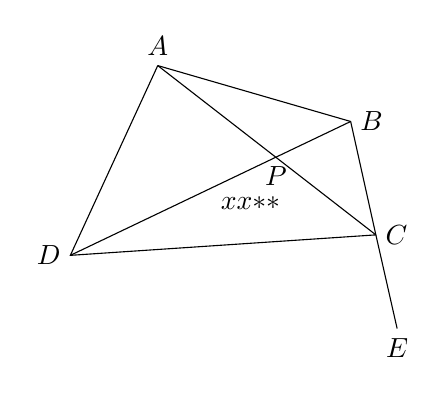
\begin{tikzpicture}
      \coordinate [label=above:$A$] (A) at (-0.8,1.83);
      \coordinate [label=right:$B$] (B) at (1.65,1.12);
      \coordinate [label=right:$C$] (C) at (1.97,-0.32);
      \coordinate [label=left:$D$] (D) at (-1.91,-0.58);
      \coordinate [label=below:$E$] (E) at (2.24,-1.51);
      
      \coordinate [label=below:$P$] (P) at (0.7,0.67);
      \coordinate (O) at (0,0);
      
      \draw (A) -- (B) -- (C) -- (D) -- (A);
      \draw (A) -- (C);
      \draw (D) -- (B);
      \draw (C) -- (E);
     
      \tkzLabelAngle[pos=0.3](D,A,C){$x$}; 
      \tkzLabelAngle[pos=0.3](D,B,C){$x$}; 
      \tkzLabelAngle[pos=0.4](A,B,D){$*$}; 
      \tkzLabelAngle[pos=0.4](A,C,D){$*$}; 
      \tkzMarkAngle[size=0.5cm,arc=l,mark=none](B,D,A);
      \tkzMarkAngle[size=0.5cm,arc=l,mark=none](B,C,A);
      \tkzMarkAngle[size=0.8cm,arc=ll,mark=none](C,A,B);
      \tkzMarkAngle[size=0.8cm,arc=ll,mark=none](C,D,B);
      
      \tkzDrawCircle(O,A);
    \end{tikzpicture}
}
\parbox[][][t]{.03\linewidth}{\hspace{.03\linewidth}}
\parbox[][][t]{.67\linewidth}{
 Sea $ABCD$ un CC tal que sus diagonales se cortan en $P \Longrightarrow$
 \begin{itemize}
     \item[i $\cdot\hspace{0.05cm}\text{-}$] $\measuredangle ABD = \measuredangle ACD$, $\measuredangle DBC = \measuredangle DAC$, etc
     \item[ii $\cdot\hspace{0.05cm}\text{-}$] $\measuredangle DAB = \measuredangle DCE$ (siendo $B$, $C$ y $E$ alineados)
     \item[iii $\cdot\hspace{0.05cm}\text{-}$] $\overline{AP}\cdot\overline{PC} = \overline{DP}\cdot\overline{PB}$ (potencia de un punto PP)
     \item[iv $\cdot\hspace{0.05cm}\text{-}$] $\overline{AB}\cdot\overline{CD} + \overline{BC}\cdot\overline{DA} = \overline{AC}\cdot\overline{BD}$ (Teorema de Ptolomeo)
     \item[v $\cdot\hspace{0.05cm}\text{-}$] $A_{ABCD} = \sqrt{p(p-a)(p-b)(p-c)(p-d)}$ ($p$ semiperímetro)
 \end{itemize}
}

\noindent y muchas otras relaciones, y como sabemos, la Geometría es el arte de relacionar elementos de las figuras presentadas.

\vspace{0.5cm}
\noindent 2) Potencia de un punto: Puede presentarse de varias formas, ver que en 1.iii $\triangle APB \sim \triangle CPD$, esta sería la primera forma.

\vspace{0.5cm}
forma 2)


\noindent\parbox[][][t]{.3\linewidth}{
    \begin{tikzpicture}
      \coordinate [label=left:$A$] (A) at (-1.91, -0.58);
      \coordinate [label=below right:$B$] (B) at (2, 0.02);
      \coordinate [label=right:$C$] (C) at (3.02,0.17);
      \coordinate [label=above right:$D$] (D) at (1.24, 1.57);
      \coordinate (E) at (0.29,2.32);
      
      \coordinate (O) at (0,0);
      
      \draw (A) -- (B) -- (C) -- (D) -- (A);
      \draw[dashed] (D) -- (B);
      \draw (D) -- (E);
   
      \tkzMarkAngle[size=0.8cm,arc=l,mark=none](C,A,D);
      \tkzMarkAngle[size=0.8cm,arc=l,mark=none](B,D,C);
   
      \tkzDrawCircle(O,A);
    \end{tikzpicture}
}
\parbox[][][t]{.2\linewidth}{\hspace{.03\linewidth}}
\parbox[][][t]{.5\linewidth}{
 Si $\overline{CD}$ tangente en $D$\\
 $\Longrightarrow \overline{DC}^2 = \overline{AC}\cdot\overline{BC}$\\
 Vea que  $\triangle ACD \sim \triangle DBC$
}

\newpage
forma 3)
\vspace{0.3cm}

\noindent\parbox[][][t]{.3\linewidth}{
    \begin{tikzpicture}
      \coordinate [label=above left:$A$] (A) at (-1.54,1.28);
      \coordinate [label=below left:$B$] (B) at (-0.5,-1.94);
      \coordinate [label=below:$C$] (C) at (-0.2,-2.85);
      \coordinate [label=below right:$D$] (D) at (0.31,-1.98);
      \coordinate [label=above right:$E$] (E) at (1.87,0.7);
      
      \coordinate (O) at (0,0);
      
      \draw (A) -- (B) -- (C) -- (D) -- (E);
      \draw[dashed] (E) -- (B);
      \draw[dashed] (A) -- (D);
      
      \tkzMarkAngle[size=1.5cm,arc=l,mark=none](C,A,D);
      \tkzMarkAngle[size=1.5cm,arc=l,mark=none](B,E,C);
   
      \tkzDrawCircle(O,A);
    \end{tikzpicture}
}
\parbox[][][t]{.2\linewidth}{\hspace{.03\linewidth}}
\parbox[][][t]{.5\linewidth}{
 $\overline{CE}\cdot\overline{DC} = \overline{CA}\cdot\overline{BC}$\\
 Vea que  $\triangle ACD \sim \triangle BCE$
}

\vspace{0.3cm}

\noindent 3) Eje radical de dos circunferencias (ER)

Veamos las formas de presentarse

\vspace{0.5cm}

\noindent\parbox[][][t]{.45\linewidth}{
forma 1

\begin{center}
Circunferencias Tangentes\\
Externas    
\end{center}

\vspace{0.5cm}

    \begin{tikzpicture}
      \coordinate [label=below:$O_1$] (O1) at (-2.5, 0);
      \coordinate [label=below:$O_2$] (O2) at (2, 0);
      \coordinate [label=below:] (P) at (-1,0);
      \coordinate [label=below right:] (E) at (-1,2.5);
      \coordinate [label=below:$ER$] (R) at (-1,-3);
      
      \filldraw (O1) circle[radius=1.5pt];
      \filldraw (O2) circle[radius=1.5pt];
      
      \draw[dashed] (O1) -- (O2);
      \draw (E) -- (R);
      
      \tkzMarkRightAngle(O1,P,E);
      
      \tkzDrawArc[angles,color=black](O1,P)(-90,150)
      \tkzDrawArc[angles,color=black](O2,P)(100,-80)
    \end{tikzpicture}
}
\parbox[][][t]{.1\linewidth}{\hspace{.1\linewidth}}
\noindent\parbox[][][t]{.45\linewidth}{
forma 2

\begin{center}
Circunferencias\\
Exteriores    
\end{center}

\vspace{0.5cm}

    \begin{tikzpicture}
      \coordinate [label=below:$O_1$] (O1) at (-2.5, 0);
      \coordinate [label=below:$O_2$] (O2) at (2, 0);
      \coordinate [label=below:] (P) at (-1,0);
      \coordinate [label=below:] (P1) at (-1.5,0);
      \coordinate [label=below:] (P2) at (-0.8,0);
      \coordinate [label=below right:] (E) at (-1,2.5);
      \coordinate [label=below:$ER$] (R) at (-1,-3);
      
      \filldraw (O1) circle[radius=1.5pt];
      \filldraw (O2) circle[radius=1.5pt];
      
      \draw[dashed] (O1) -- (O2);
      \draw (E) -- (R);
      
      \tkzMarkRightAngle(O1,P,E);
      
      \tkzDrawArc[angles,color=black](O1,P1)(-140,150)
      \tkzDrawArc[angles,color=black](O2,P2)(70,-60)
    \end{tikzpicture}
}

\vspace{0.5cm}

\noindent\parbox[][][t]{.45\linewidth}{
forma 3

\begin{center}
Circunferencias Tangentes\\
Interiores    
\end{center}

\vspace{0.5cm}

    \begin{tikzpicture}
      \coordinate [label=below:$O_1$] (O1) at (0.1, 0);
      \coordinate [label=below:$O_2$] (O2) at (1.5, 0);
      \coordinate [label=below:] (P) at (-1.5,0);
      \coordinate [label=below right:] (E) at (-1.5,3);
      \coordinate [label=below:$ER$] (R) at (-1.5,-3);
      
      \filldraw (O1) circle[radius=1.5pt];
      \filldraw (O2) circle[radius=1.5pt];
      
      \draw[dashed] (O2) -- (P);
      \draw (E) -- (R);
      
      \tkzMarkRightAngle(O1,P,E);
      
      \tkzDrawCircle(O1,P);
      \tkzDrawCircle(O2,P);
    \end{tikzpicture}
}
\parbox[][][t]{.1\linewidth}{\hspace{.1\linewidth}}
\noindent\parbox[][][t]{.45\linewidth}{
forma 4

\begin{center}
Circunferencias\\
Secantes    
\end{center}

\vspace{0.5cm}

    \begin{tikzpicture}
      \coordinate [label=below:$O_1$] (O1) at (-3, 0);
      \coordinate [label=below:$O_2$] (O2) at (1, 0);
      \coordinate [label=below:] (P) at (-1.68,0);
      \coordinate [label=right:$A$] (A) at (-1.68,1.54);
      \coordinate [label=right:$B$] (B) at (-1.68,-1.54);
      \coordinate [label=below right:] (E) at (-1.68,3.5);
      \coordinate [label=below:$ER$] (R) at (-1.68,-3);
      
      \coordinate [label=below right:$P$] (PP) at (-1.68,3);
      \coordinate [label=below:$Q$] (QQ) at (-3.95,1.79);
      \coordinate [label=below:$R$] (RR) at (0.89,3.09);
      
      \filldraw (O1) circle[radius=1.5pt];
      \filldraw (O2) circle[radius=1.5pt];
      
      \draw[dashed] (O1) -- (O2);
      \draw (E) -- (R);
      \draw (QQ) -- (PP);
      \draw (PP) -- (RR);
      
      \tkzMarkRightAngle(O1,P,E);
      
      \tkzDrawArc[angles,color=black](O1,A)(-140,150)
      \tkzDrawArc[angles,color=black](O2,A)(70,-60)
    \end{tikzpicture}
}